\chapter{The Stability of Conceptual Models of the Carbon Cycle}
\label{chapter:conceptual_carbon_cycle}
\graphicspath{{box_ocean/figs/}}

\lettrine[lines=3,loversize=0.1,findent=0.1em,nindent=0em]{I}{n} \cref{chapter:global_bomb}, I adapted a result of~\cite{Cox2006}
which showed that there were conditions under which the pre-industrial state of the carbon-climate
system was unstable. This instability was driven by the terrestrial carbon cycle. That analysis involved representing the effect of the ocean as taking up a fixed fraction,
$\chi_0$, of carbon emissions to the atmosphere. This neglects any dynamical role of the ocean, including processes that occur on different timescales. Furthermore that analysis
made inconsistent assumptions about the pre-industrial climate. This chapter will update~\cite{Cox2006}, by constructing a model of the climate-carbon system with a dynamical ocean component
that is consistent about the pre-industrial state.

I will neglect the role of biogeochemical heating as \cref{chapter:global_bomb} found it a small effect at the global scale.

\section{Background}

\subsection{Climate Response to Radiative Forcing}
As was outlined in \cref{sec:intro1}, the climate system responds to increasing levels of greenhouse gases in the atmosphere by increasing in temperature. The radiative forcing
forcing and associated temperature rise caused by doubling the concentration of \ce{CO2} in the atmosphere is generally assumed to be state independent. The amount of warming
in the global mean caused by doubling \ce{CO2} is known as the equilibrium climate sensitivity, $\mathrm{ECS}$, and is
\SI{3.0}{\kelvin} with a likely range of \SIrange{2.5}{4.0}{\kelvin} \parencite{AR6,Sherwood2020}.
However the latest generation CMIP6 climate models have climate sensitivities up to \SI{5.6}{\kelvin} \parencite{Zelinka2020} and some climate models can give sensitivities of over
\SI{11}{\kelvin} \parencite{Stainforth2005}.

It should also be noted that the warming is not globally uniform, with land warming more than the oceans \parencite{Morice2021} and higher latitudes warming more than the tropics \parencite{Serreze2011}.
This enhanced warming in the Arctic is known as `Arctic amplification'. A common approximation is `pattern scaling' which related the spatially dependent warming, $\Delta T(\bm{r},t)$
to the change in global mean surface temperature $\Delta T(t)$ by a time invariant pattern of warming, $f(\bm{r})$,
through $\Delta T(\bm{r},t) = f(\bm{r}) \Delta T(t)$ \parencite{Huntingford2000a}.



\subsection{Terrestrial Carbon Cycle Response to \ce{CO2}}
Whilst the above discussion of $\mathrm{ECS}$ treats the amount of $\ce{CO2}$ in the atmosphere as a given quantity, in reality it is also affected by the climate
system, which determines the fluxes of carbon into and out of the atmosphere through biogeochemical cycles \parencite{Rothman2014}.

One important feedback is the so-called Jenkinson effect \parencite{Jenkinson1991} which is enhanced heterotrophic respiration due to elevated surface temperatures. This
tends to increase the amount of \ce{CO2} in the atmosphere and so it is a positive feedback on climate change.

At higher levels of \ce{CO2}, the net primary productivity (NPP) of vegetation increases, this effect is called the \ce{CO2} fertilisation effect \parencite{Wenzel2016}.
This tends to decrease the levels of \ce{CO2} in the atmosphere and is thus a negative feedback on climate change.

The net effect of these two feedbacks is that the terrestrial response to \ce{CO2} is uncertain as the sign of the response depends on the relative magnitude of these effects. Overall it
is thought that \ce{CO2} fertilisation dominates at lower \ce{CO2} levels, which is consistent with the observed carbon sink, however at higher \ce{CO2} levels the Jenkinson effect
dominates \parencite{Cox2000,Friedlingstein2006,Arora2020}.

\subsection{Potential For Instability}
Combining these two sensitivities gives the potential for an instability. Consider the following situation. Suppose some carbon is transferred from the land to the atmosphere. Then the Earth
will warm. Due to positive feedbacks from the land more carbon will be released into the atmosphere leading to further warming and more carbon released. This cycle could continue until all the
carbon from the land has been released into the atmosphere. However, because of the negative feedbacks in the system (principally \ce{CO2} fertilisation) these positive feedbacks would have to be
sufficiently strong in order for this to happen.

The fact that there is carbon on land \parencite{Crowther2019} combined with the small variation in atmospheric \ce{CO2} over the pre-industrial Holocene \parencite{Marcott2014,Bauska2015},
therefore indicates something about the magnitudes of the land carbon feedback and the climate sensitivity, namely that they cannot be too large.
To make progress analysing this we must include the effect of the other store of carbon: the ocean.

\section{A Climate-Carbon Cycle model using IMOGEN as the Ocean Component}
\subsection{IMOGEN description}
The land surface model JULES is often used in conjunction with IMOGEN \parencite{Huntingford2004,Huntingford2010} which is a model that `closes' the carbon cycle in that it provides
an atmospheric and oceanic response to changes in terrestrial carbon. In this chapter, the ocean component of IMOGEN will be isolated. The ocean component is based on the
model of~\cite{Joos1996} which represents ocean carbon in terms of an impulse response to atmospheric \ce{CO2}.

It calculates the changes in dissolved inorganic carbon in the surface water as
\begin{equation}
  \label{eq:imogen_upper_ocean_carbon}
  \delta \Sigma \ce{CO2} = \int_0^{t} F_{a}(t-s)G_{I}(s)\dd{s}.
\end{equation}
where $F_a$ is the atmosphere to ocean flux of carbon and $G_I$ is IMOGEN's impulse-response function. This function is defined as
\begin{equation}
  \label{eq:imogen_impulse_response}
  G_I(t) =
  \begin{cases}
    1 - 2.2617t + 14.002t^2 - 48.770t^3 & t \leq \SI{1}{\year} \\
    f_0 + \sum_{i=1}^{5} f_i e^{-t/\tau_i} & t > \SI{1}{\year}
  \end{cases}
\end{equation}
where $f_0=0.014819,f_1 = 0.70367,f_2=0.24966,f_3=0.066485,f_4 = 0.038344,f_5=0.019439$ and $\tau_1= 0.70177,\tau_2 = 2.3488,\tau_3=15.281,\tau_4 = 65.359,\tau_5 = 347.55$, the $\tau_i$ have units of
years. This function is dimensionless and plotted in \cref{fig:imogen_impulse_response}.

\begin{figure}
  \centering
  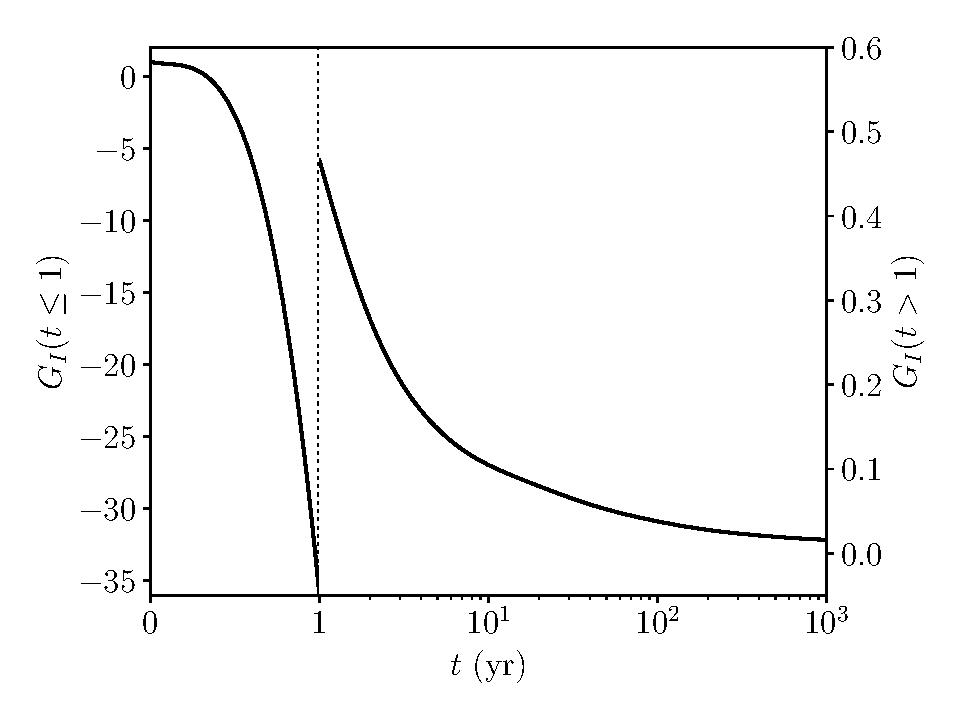
\includegraphics[width=\textwidth,keepaspectratio]{GI}
  \caption[IMOGEN's impulse-response function]{The impulse-response function for the ocean carbon uptake in IMGOEN, described by \cref{eq:imogen_impulse_response}. The function is discontinuous at $t = \SI{1}{\year}$. The dotted line indicates this discontinuity. Note the differences in scales on both the $x$ and $y$ axes either side of this discontinuity.}
  \label{fig:imogen_impulse_response}
\end{figure}

The carbon flux is given by
\begin{equation}
  \label{eq:imogen_ocean_atmosphere_flux}
  F_a(t) = k \left(\Delta C_a - \Delta C_o\right)
\end{equation}
where $\Delta C_a$ and $\Delta C_o$ are the perturbations in atmospheric and ocean carbon. To take into account ocean temperature feedbacks on the ocean carbon cycle $\Delta C_o$ and
$\delta \Sigma \ce{CO2}$ are related by
\begin{equation}
  \label{eq:imogen_temp_feedback}
  \Delta C_o = g(T_o,\delta \Sigma \ce{CO2})e^{0.0423\Delta T_o}
\end{equation}
where $T_o$ is the initial ocean temperature, $\Delta T_o$ is the change in ocean temperature and $g$ is a quintic polynomial in $\delta \Sigma \ce{CO2}$ whose coefficients depend on $T_o$.
\subsection{Terrestrial Carbon Cycle}
The total carbon in the carbon cycle is a constant given by $\mathcal{C}  = C_s + C_a + C_o$ where $C_s$ is the soil carbon, $C_a$ is the atmospheric carbon  and $C_o$ is the ocean carbon.
Therefore to close the system, given the ocean dynamics, only the land carbon dynamics need to be set, with the dynamics of atmospheric carbon being controlled by this conservation law.

The change in soil carbon is given by the difference between net primary productivity and heterotrophic respiration. Heterotrophic
respiration is assumed to have the following form:
\begin{equation}
  \label{eq:heterotrophic_respiration}
  R_h = r_0 C_s Q_{10}^{\Delta T_a/10} = r_0 C_s e^{\alpha \Delta T_a}
\end{equation}
where $\Delta T_a$ is the change in atmospheric temperature, $r_0$ is a reference respiration level and $\alpha = 0.1\log Q_{10}$ is the strength of the temperature feedback.

It is assumed that $\Delta T_a$ depends logarithmically on atmospheric carbon
\begin{equation}
  \label{eq:air_temperature}
  \Delta T_a = \frac{S}{\log 2} \log \frac{C_a}{C_{a0}}
\end{equation}
where $C_{a0}$ is a reference \ce{CO2} level, set at \SI{589}{\peta\gram\carbon}, which is approximately the pre-industrial
level of \ce{CO2} \parencite{Lade2018}. The parameter $S$ is an NPP weighted climate sensitivity, as shown in
\cref{chapter:global_bomb}. This could be larger than $\mathrm{ECS}$ by a factor of about $1.5$, estimates of $S/\mathrm{ECS}$ are given
in \cref{tab:S_vs_ECS}. \Cref{eq:heterotrophic_respiration} can be combined with \cref{eq:heterotrophic_respiration} to give
\begin{equation}
  R_h = r_0 C_s e^{\frac{\alpha S}{\log 2} \log \frac{C_a}{C_{a0}}} = r_0 C_s \exp\left(\log \left( \left(\frac{C_a}{C_{a0}}\right)^{\frac{\alpha S}{\log 2}}\right)\right)
\end{equation}
or
\begin{equation}
  \label{eq:heterotrophic_respiration_combined}
  R_h = r_0 C_s \left( \frac{C_a}{C_{a0}}\right)^{\mu}
\end{equation}
where
\begin{equation}
  \label{eq:mu}
  \mu = \frac{1}{\log 2} \alpha S.
\end{equation}

\begin{table}
   \centering
   \begin{tabular}{llll}
     \toprule
     \multicolumn{2}{c}{CMIP5}               & \multicolumn{2}{c}{CMIP6}            \\
     Model              & $S/\mathrm{ECS}$ & Model       & $S/\mathrm{ECS}$         \\
     \midrule
     BCC-CSM1-1         & $1.1$            & BCC-CSM2-MR     & $1.4$               \\
     BCC-CSM1-1-M       & $1.4$            & BCC-ESM1        & $1.2$               \\
     BNU-ESM            & $1.4$            & CanESM5         & $1.2$               \\
     CanESM2            & $1.4$            & CAS-ESM2-0      & $1.4$               \\
     IPSL-CM5A-LR       & $1.6$            & CESM2           & $1.1$               \\
     IPSL-CM5A-MR       & $1.7$            & CESM2-FV2       & $1.3$               \\
     IPSL-CM5B-LR       & $1.7$            & CESM2-WACCM     & $1.3$               \\
     MIROC-ESM          & $1.6$            & CESM2-WACCM-FV2 & $1.2$               \\
     HadGEM2-ES         & $1.3$            & CMCC-CM2-SR5    & $1.6$               \\
     MPI-ESM-LR         & $1.4$            & CMCC-ESM2       & $1.6$               \\
     MPI-ESM-MR         & $1.5$            & GFDL-ESM4       & $1.3$               \\
     MPI-ESM-P          & $1.6$            & NorCPM1         & $1.2$               \\
     GISS-E2-H          & $1.5$            & GISS-E2-1-G     & $1.5$               \\
     GISS-E2-R          & $1.6$            & GISS-E2-1-H     & $1.5$               \\
     CCSM4              & $1.3$            & GISS-E2-2-G     & $1.4$               \\
     NorESM1-M          & $1.3$            & GISS-E2-2-H     & $1.5$               \\
     GFDL-ESM2G         & $1.6$            & INM-CM4-8       & $1.4$               \\
     GFDL-ESM2M         & $1.5$            & INM-CM5-0       & $1.4$               \\
                        &                  & IPSL-CM5A2-INCA & $1.9$               \\
                        &                  & IPSL-CM6A-LR    & $1.2$               \\
                        &                  & NorESM2-LM      & $1.2$               \\
                        &                  & NorESM2-MM      & $1.3$               \\
                        &                  & TaiESM1         & $1.3$               \\
                        &                  & UKESM1-0-LL     & $1.3$               \\
     Ensemble Mean      & $1.5 \pm 0.2$    & Ensemble Mean   & $1.4\pm0.2$         \\
     \bottomrule
   \end{tabular}
\caption[Estimates of $S/\mathrm{ECS}$ for CMIP models]{Estimates of the ratio of $S$ to $\mathrm{ECS}$ for CMIP5 and CMIP6 models, calculated by the methodology described in \cref{chapter:global_bomb}.
  The ensemble mean is given plus or minus one standard deviation.}
\label{tab:S_vs_ECS}
\end{table}

Following \cite{Cox2006}, net primary productivity is modelled as
\begin{equation}
  \label{eq:npp}
  \Pi(C_a) = \Pi_{\infty}\frac{C_a}{C_a + C_{1/2}},
\end{equation}
which is an increasing function of \ce{CO2} that saturates for $C_a \gg C_{1/2}$. Unless otherwise stated, $C_{1/2} = \SI{280}{\ppm}$, which is compatible with other estimates
\parencite{KolbySmith2016,Wenzel2016}. This parameter controls the strength of the \ce{CO2} fertilisation feedback. \Cref{eq:npp} assumes that net primary productivity depends only
on \ce{CO2}. Allowing for other factors like nitrogen limitation would act to reduce the effective $C_{1/2}$ value. $\Pi_{\infty}$ is set so that $\Pi_0 = \Pi(C_{a0})$ is the pre-industrial
level of net primary productivity \SI{55}{\peta\gram\carbon\per\year} \parencite{Lade2018}.

Putting this all together leads to the following set of coupled differential equations:
\begin{subequations}
  \label{eq:imogen_deterministic}
  \begin{align}
    \dv{C_s}{t}     &= \Pi(C_a) - C_s r_0 \left(\frac{C_a}{C_{a0}}\right)^\mu \\
    \dv{C_o}{t}     &= I(C_a,\Delta T_o,C_o) \\
    C_a             &= \mathcal{C} - C_s - C_o \\
    \Delta T_o             &= \frac{1}{\nu}\frac{S}{\log 2}\log \frac{C_a}{C_{a0}}.
  \end{align}
\end{subequations}
The function $I$ represents the IMOGEN model, $\Delta T_o$ is the change in ocean temperature which is related to the change in land temperature by the
factor $\nu = 1.45$. Note that $S$ and $Q_{10}$ (through $\mu$) appear separately in this equation, so both parameters will affect the bifurcation point.

Note that there is an equilibrium at $C_a = C_{a0}$, $C_s = C_s^{\mathrm{eq}} = \Pi(C_{a0})/r_0$, $C_o = 0$, $\Delta T_o = 0$, corresponding to the pre-industrial equilibrium, which has been
experienced only small variations over the (pre-industrial) Holocene.

\subsection{Bifurcations in IMOGEN}
\Cref{eq:imogen_deterministic} is solved for a range of values of $S$ with $Q_{10} = 2$. The system was initialised close to equilibrium and then allowed to equilibrate over 5000 years.
The results for atmospheric carbon are plotted in \cref{fig:imogen_trajectories}. For values of $S$ between \SIrange{10}{11}{\kelvin} there is a
transition to oscillatory behaviour. In \cref{sec:two_box} this will be shown to be caused by a Hopf bifurcation.
\begin{figure}
  \centering
  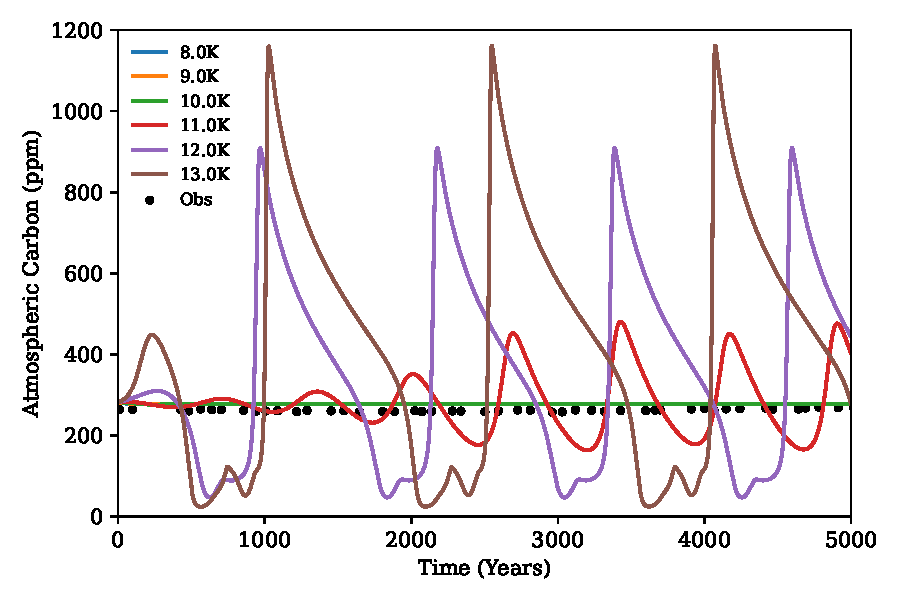
\includegraphics[width=\textwidth,keepaspectratio]{imogen_traj}
  \caption[Using IMOGEN to find the behaviour of atmospheric \ce{CO2} for various values of $S$]{Atmospheric carbon calculated with the IMOGEN model
    given by \cref{eq:imogen_deterministic} for a range of $S$ values,
    with $Q_{10} = 2$. Overlaid are measurements of early Holocene (\SIrange{10000}{5000}{\year\beforepresent}) \ce{CO2} levels, taken from~\cite{Bereiter2015}.
  Note that large $S$ values lead to behaviour incompatible with the observed atmospheric \ce{CO2} record.}
  \label{fig:imogen_trajectories}
\end{figure}

To scan the parameter space, this IMOGEN model was used to estimate the critical $S$ as a function of $Q_{10}$ and $C_{1/2}$,
the parameter that controls the \ce{CO2} fertilisation effect. This is plotted in \cref{fig:imogen_bifurcation_plane}.

\begin{figure}
  \centering
  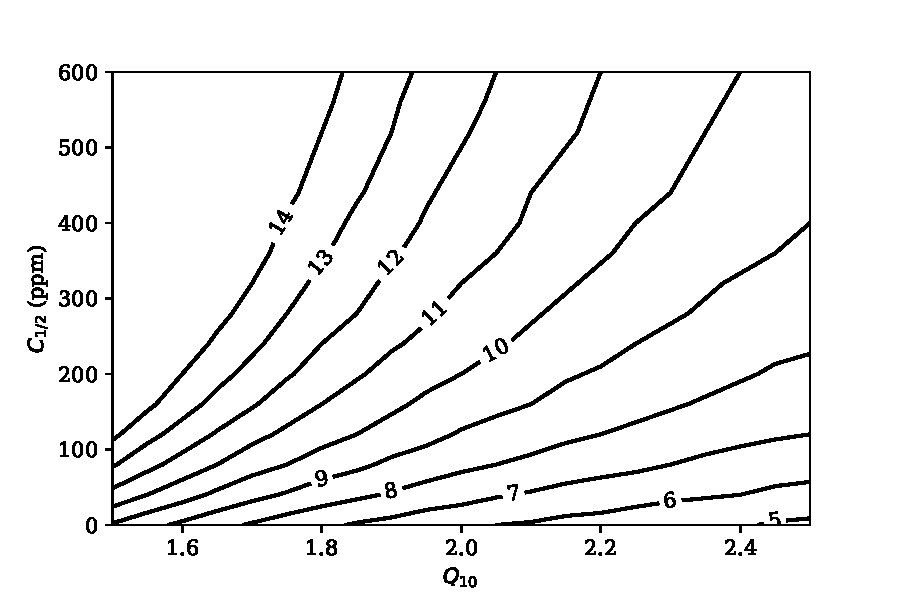
\includegraphics[keepaspectratio,width=\textwidth]{imogen_critical_S_Q10_ca05}
  \caption[The dependence of the critical values of $S$ on $Q_{10}$ and $C_{1/2}$]{A contour plot showing the value of $S$ as a function of $Q_{10}$ (the temperature dependence of respiration)
    and $C_{1/2}$ (the strength of the \ce{CO2} fertilisation
    feedback) at which the Hopf bifurcation occurs in \cref{eq:imogen_deterministic}.
    Values of $S$ larger than  this are incompatible with the observed behaviour of the carbon cycle.}
  \label{fig:imogen_bifurcation_plane}
\end{figure}

As some CMIP6 models have an $S \approx\SI{9}{K}$ this imposes limits on the strength of their carbon cycle feedbacks. Furthermore, because these models are
near this bifurcation point, they will be subject to critical slowing down. This could lead to unrealistic \ce{CO2} variability, even if they are
in the non-oscillatory branch of the carbon cycle.

Despite the simplicity of this model, it is still too complex to analyse mathematically. In the next section a simplified model will be developed to enable this bifurcation to be investigated further.

\section{A Simpler Ocean Model}
This simpler model will neglect temperature feedbacks on the ocean response. Further assumed is that the ocean carbon carbon uptake
can be viewed as $N$ non-interacting boxes which each respond over a timescale $\tau_i$ where $i$ indexes the boxes. A fraction $f_i$ of the total carbon
flux will enter the $i$th box. These assumptions can be justified in that they represent a simplification of the IMOGEN model and can be used to fit the observed ocean carbon
uptake, which is done in \cref{sec:ocean_uptake}.

The model is as follows: the change in carbon stored in the $i$th box, $C_i$, is given by
\begin{equation}
  \label{eq:ocean_box_i}
  \dv{C_i}{t} = f_ik \Delta C_a(t) - \frac{C_i}{\tau_i},
\end{equation}
where $k=\SI{0.2}{\per\year}$ gives the timescale of the ocean uptake and $\Delta C_a$ is the change in atmospheric carbon from its equilibrium value.

For a given $C_a(t)$ \cref{eq:ocean_box_i} can be solved in quadratures to give
\begin{equation}
  \label{eq:solution_for_box_i}
  C_i(t) = \int_0^t f_ik e^{-s/\tau_i} \Delta C_a(t - s) \dd{s},
\end{equation}
where $C_i(0) = 0$.

The overall ocean response is therefore
\begin{equation}
  \label{eq:ocean_response}
  \Delta C_o(t) = \sum_{i=1}^N \int_0^t f_ik e^{-s/\tau_i} \Delta C_a(t - s) \dd{s}.
\end{equation}
or
\begin{equation}
  \label{eq:ocean_response_in_terms_of_G}
  \Delta C_o(t) = \int_0^t G(s) \Delta C_a(t-s) \dd{s}
\end{equation}
where
\begin{equation}
  \label{eq:ocean_greens_function}
  G(t) = \sum_{i=1}^{N} f_ik e^{-t/\tau_i}
\end{equation}
is the impulse response function for the uptake of ocean carbon. It is assumed that $\Delta C_a(t) = 0$  for $t < 0$, and thus the lower bound
of integration can be set to zero. \Cref{eq:oceans_greens_function} is similar to \cref{eq:imogen_impulse_response}, except the short term behaviour differs qualitatively
and there is no nonlinear dependence on ocean carbon.

\section{One Box Ocean}
The simplest possible ocean box model is a one box model. This will be analysed first to see if it can reproduce the results of the IMOGEN model.

The one box model can be written symbolically through the following set of ODEs
\begin{subequations}
  \label{eq:one_box_ocean}
  \begin{align}
    \dv{C_s}{t} &= \Pi(C_a) - r_0 C_s \left(\frac{C_a}{C_{a0}}\right)^{\mu} \\
    \dv{C_o}{t} &= k(C_a - C_{a0}) - \frac{C_o}{\tau} \\
    C_a &= \mathcal{C} - C_s - C_o.
\end{align}
\end{subequations}
Note that unlike the IMOGEN case the dependence on $Q_{10}$ and $S$ is combined into one parameter $\mu$. Again, there is a fixed point at
$C_a = C_{a0}$, $C_o = 0$ and $C_s = C_s^{\mathrm{eq}}$.

\subsection{Stability of Pre-industrial State in One Box Model}
As shown in \cref{sec:btipping}, a fixed point of a system is unstable when the Jacobian, $J$, of that system evaluated at the fixed point has an eigenvalue, $\gamma$, with a positive real part.
The Jacobian of \cref{eq:one_box_ocean} is given by
\begin{equation}
  \label{eq:jacobian_of_one_box}
    J = 
    \begin{pmatrix}
    r_0 \left( \mu \frac{C_s^{\mathrm{eq}}}{C_{a0}} - 1\right) - \Pi'(C_{a0}) & 
    \mu \frac{C_s^{\mathrm{eq}}}{C_{a0}} - \Pi'(C_{a0}) \\
    -k & -k - \frac{1}{\tau}
    \end{pmatrix}
  \end{equation}
where $\Pi'(C_a)$ denotes the derivative of NPP with respect to atmospheric carbon.
  
To find the eigenvalues of the Jacobian, the characteristic polynomial
\begin{equation}
  \label{eq:char_poly}
  \det(J - \gamma I) = 0
\end{equation}
must be solved for $\gamma$.

This equation is quadratic and therefore has two roots. Solving it leads to a solution of the form:
\begin{equation}
  \label{eq:eigenvalues_of_one_box_jac}
  \gamma_{\pm} = \frac{B \pm \sqrt{D}}{2\tau C_{a0}}
\end{equation}
where
\begin{equation}
  \label{eq:B_in_one_box}
  B = -k \tau  C_{a0}-\Pi'(C_{a0}) \tau  C_{a0}-r_0 \tau  C_{a0}-C_{a0}+\mu  \Pi_0 \tau
\end{equation}
and
\begin{equation}
  \label{eq:discriminant_from_one_box}
  D = C_{a0}^2\tau^2\left(\left(k +\Pi' +r_0  +\frac{1}{\tau}-\frac{\mu  \Pi_0}{C_{a0}} \right)^2-\frac{4}{\tau}\left(k r_0 \tau +\Pi'+r_0-\frac{\mu  \Pi_0}{C_{a0}}\right)\right)
\end{equation}
is the discriminant and the substitution $\Pi_0 = r_0 C_s^{\mathrm{eq}}$ has been made.

The stability of this system is governed by $\Re \gamma$. This number is controlled by the sign of $D$. If $D > 0$, then $\gamma$ is purely real, but if $D < 0$, then
$\Re \gamma = B / 2\tau C_{a0}$. 

\subsection{Real Eigenvalues}
If $\tau < 1/r_0$ then $D > 0$ for all values of $\mu$. As $1/r_0 = C_s^{\mathrm{eq}}/\Pi_0 \approx \SI{30}{\year}$ this situation represents a relatively fast ocean response.
Under this assumption, it turns out that $\gamma_+ > 0$ when
\begin{equation}
  \label{eq:instability_condition_one_box_fast}
  \mu^* = \frac{C_{a0}}{C_s^{\mathrm{eq}}} + \frac{C_{a0}}{\Pi_0} \dv{\Pi}{C_a} + \frac{C_{a0}}{C_s^{\mathrm{eq}}} k\tau.
\end{equation}
It is interesting to compare this to the condition given in \cref{eq:mu_infinity}. If the parameter $\chi_0$ is introduced, as by~\cite{Cox2006}, and set to $\chi_0 = k \tau$,
then \cref{eq:instability_condition_one_box_fast} is identical to \cref{eq:mu_infinity}. This gives an interpretation to $\chi_0$ as the ratio of the timescale of the ocean carbon flux
to the timescale of its response. Previously, $\chi_0$ was interpreted as a fraction. This can be done only if $\tau < 1/k = \SI{5}{\year}$.
\begin{figure}
  \centering
  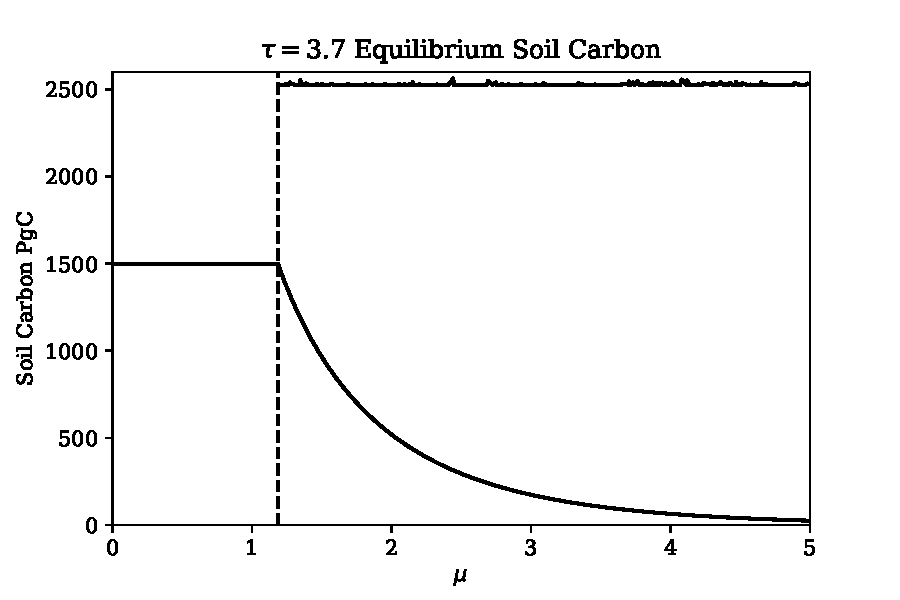
\includegraphics[keepaspectratio,width=\textwidth]{one_box_model_soil_carbon_equilibrium_tau_3.7}
  \caption[One box soil carbon equilibrium]{Equilibrium levels of soil carbon as a function of $\mu$ for the one box ocean model, \cref{eq:one_box_ocean},
    calculated numerically. The ocean timescale is \SI{3.7}{\year}, which is in the fast ocean response regime.
    The dashed line is the analytically calculated bifurcation point, \cref{eq:instability_condition_one_box_fast}.}
  \label{fig:fast_response_bf_diagram}
\end{figure}

The system \cref{eq:one_box_ocean} is integrated to equilibrium and the equilibria are plotted as a function of $\mu$ in \cref{fig:fast_response_bf_diagram},
with $\tau = \SI{3.7}{\year}$. The dashed line represents the position of the analytically calculated bifurcation point.
It can been seen that the agreement is good, and that this is a transcritical bifurcation.

\subsection{Complex Eigenvalues}
In the case where the ocean timescale is larger than $1/r_0$, then $D < 0$. This means if the ocean response is considered to have a long timescale,
the stability of the system is given by the sign of $B$.

The value of $B$ will become positive when $\mu$ exceeds the following threshold:
\begin{equation}
  \label{eq:instability_condition_one_box_slow}
  \mu^* =\frac{C_{a0}}{C_s^{\mathrm{eq}}} + \frac{C_{a0}}{\Pi_0} \dv{\Pi}{C_a} + \frac{C_{a0}}{C_s^{\mathrm{eq}}} k\tau\left(
     1 + \frac{1}{k\tau}
  \right) \frac{1}{r_0\tau}
\end{equation}
This is similar to the conditions derived in \cref{eq:mu_infinity,eq:instability_condition_one_box_fast} except now $\chi_0 = k\tau\left(1 + \frac{1}{k\tau} \right) \frac{1}{r_0\tau} \approx k/r_0$
where the approximation assumes $k \gg r_0$. This means the ``fraction absorbed by the oceans'' is now controlled by the ratio of the timescale of the ocean flux to the turnover time of the soil.
Furthermore because $k > r_0$, then $\chi_0$ will be larger than $1$. This means that $\chi_0$ can't be interpreted as a fraction of carbon absorbed any more.
In addition, because $\gamma$ is complex, this bifurcation occurs when the complex conjugate eigenvalue pair crosses the imaginary axis. This means this bifurcation is
a Hopf bifurcation rather than a transcritical bifurcation.
\begin{figure}
  \centering
  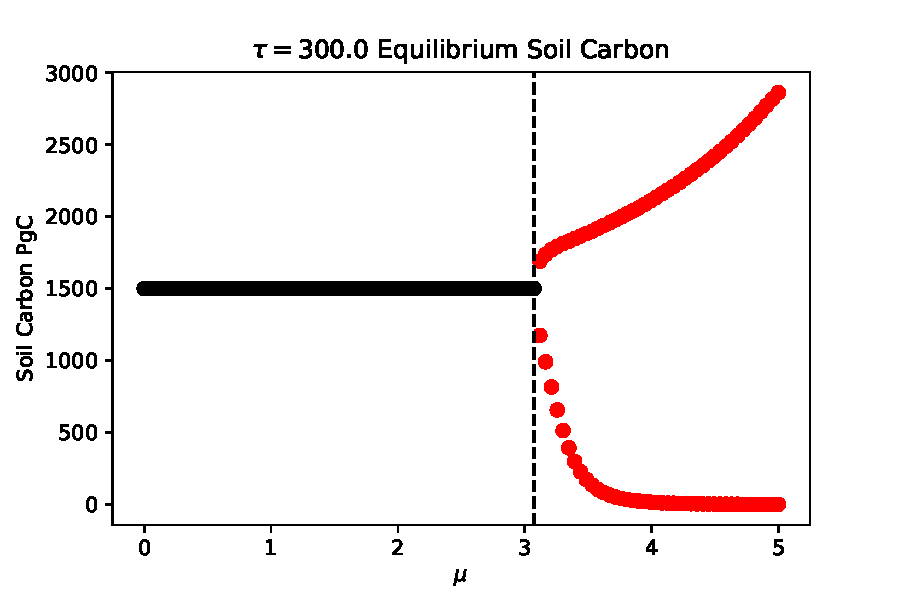
\includegraphics[keepaspectratio,width=\textwidth]{one_box_model_soil_carbon_equilibrium_tau_300.0}
  \caption[One box soil carbon equilibrium]{Equilibrium levels of soil carbon as a function of $\mu$ for the one box ocean model, \cref{eq:one_box_ocean},
    calculated numerically. The ocean timescale is \SI{300}{\year}, which is in the slow ocean response regime.
    The dashed line is the analytically calculated bifurcation point, \cref{eq:instability_condition_one_box_slow}.
    Solid black lines represent a steady state condition, whereas red lines show that maximum and minimum of an oscillatory state. The oscillation period increases almost
    linearly with $\mu$ from around \SI{23}{\year} to \SI{112}{\year}. }
  \label{fig:slow_response_bf_diagram}
\end{figure}
For the case where $\tau = \SI{300}{\year}$ \cref{eq:one_box_ocean} was integrated numerically and the equilibrium was found as a function of $\mu$,
which is plotted in \cref{fig:slow_response_bf_diagram}. Where the equilibrium is an oscillation rather than a steady state the plot shows the maximum and minimum of the
oscillation in red. It can be seen that the agreement with the numerics is good.

Based on the conditions derived in \cref{eq:instability_condition_one_box_fast,eq:instability_condition_one_box_slow} the critical value of $\mu$ can be chosen to match the
bifurcation point predicted by the IMOGEN model. This involves choosing $\tau = \SI{2.23}{\year}$. This puts the ocean into the fast regime, and therefore a transcritical bifurcation.
This is a different sort of bifurcation to the one found in IMOGEN and so motivates increasing the complexity of the ocean model slightly.

\section{Two Box Model}
\label{sec:two_box}
To improve the realism of the model, the two box ocean case is now considered. In order to do this \cref{eq:one_box_ocean} must be modified to include
two ocean stores of carbon $C_1$ and $C_2$. Each box will have their own timescale $\tau$ and $\tau/\epsilon$ respectively. This notation is suggestive of
$C_1$ being a fast box and $C_2$ being a slow box, although this restriction is not necessary.

This leads to the following system of equations:
\begin{subequations}
  \label{eq:two_box_ocean}
  \begin{align}
    \dv{C_s}{t} &= \Pi(C_a) - r_0 C_s \left(\frac{C_a}{C_{a0}}\right)^{\mu} \\
    \dv{C_1}{t} &= fk(C_a - C_{a0}) - \frac{C_1}{\tau} \\
    \dv{C_2}{t} &= (1-f)k(C_a-C_{a0}) - \epsilon\frac{C_2}{\tau} \\
    C_a &= \mathcal{C} - C_s - C_1 - C_2.
  \end{align}
\end{subequations}
Again note the equilibrium at $C_a = C_{a0}$,$C_s = C_s^{\mathrm{eq}}$ and $C_1 = C_2 = 0$. To determine the stability of this state the eigenvalues of the Jacobian
of \cref{eq:two_box_ocean} must be computed, which involves finding the roots of a cubic characteristic polynomial.
Whilst this is possible in principle it is analytically very challenging.

To avoid this therefore some heuristic arguments are given as to why a Hopf bifurcation occurs at a critical value of $\mu$. A special case of the 
characteristic polynomial of the Jacobian is solved, which corresponds to assuming the existence of a Hopf bifurcation. Under this assumption 
critical values of $\mu$ are found at which a Hopf bifurcation could occur, which is then verified with a numerical investigation.

\subsection{A Heuristic Argument}
For this section, the assumption of a timescale separation in ocean responses will be made, namely that $\epsilon \ll 1$. It has already been shown that a long timescale
single ocean box will lead to a Hopf so it is reasonable to expect that adding a faster box will not change this. A more mechanistic argument can be formulated as follows.

Due to the timescale
separation, over short timescales the slow box can be ignored and so it will behave like a one box system. As a result, it can be expected that there
is a value of $\mu$ which leads to an instability. This instability leads to a high atmospheric carbon state, but the ultimate fate of this carbon will depend on the long-time response of the oceans, in other
words on the slow box. Over these longer timescales the system can be treated as a one box model with the ocean box corresponding to the slow box.
Over these long timescales the slow ocean box will absorb the excess carbon from the atmosphere which will tend to cool the globe. As a result
the soil can once again become a sink of carbon. However eventually the soil will contain an amount $C_s^{\mathrm{eq}}$ of soil carbon, but it has already been argued that this state is unstable
and so the cycle will start again.

\subsection{Computation of Bifurcation Point}
If the assumption that there is a Hopf bifurcation can be made, then there is another mode of attack. At the Hopf bifurcation a pair of complex conjugate eigenvalues
cross the imaginary axis from the negative real part side to the positive real part side. This means that at the bifurcation, the eigenvalues are purely imaginary. It is
comparatively easy to solve a cubic equation under the assumption of imaginary roots.

The characteristic polynomial of the Jacobian of \cref{eq:two_box_ocean} will be of the form
\begin{equation}
  \label{eq:generic_cubic}
  \gamma^3 + a_1 \gamma^2 + a_2 \gamma + a_3 = 0,
\end{equation}
where $\gamma$ is an eigenvalue. As has been stated, at the Hopf bifurcation, $\gamma$ is purely imaginary so the substitution $\gamma = i\lambda$ with $\lambda \in \mathbb{R}$
can be made. Then \cref{eq:generic_cubic} becomes
\begin{equation}
  \label{eq:cubic_with_imaginary_root}
  -i\lambda^3 - a_1 \lambda^2 + i a_2 \lambda + a_3 = 0. 
\end{equation}
For this equation to be satisfied, both real and imaginary parts of \cref{eq:cubic_with_imaginary_root} must be zero. This leads to
$\lambda = \pm \sqrt{a_3/a_1}$ and $\lambda = \pm \sqrt{a_2}$. For consistency, these expressions for $\lambda$ must be equal. This requires that $a_3 = a_1a_2$.
Alternatively, both expressions for $\lambda$ can be satisfied if $\lambda = 0$. However, this leads to $\gamma = 0$ which has no non-zero imaginary part and so cannot lead to
oscillatory solutions and thus is not consistent with the assumption that there is a Hopf bifurcation.

The condition $a_1a_2=a_3$  can now be solved for $\mu$. Doing this gives two solutions.
\begin{equation}
  \label{eq:mu_two_box}
  \mu^* = \frac{C_{a0}}{2 \Pi_0 \tau  (1+\epsilon)} \left(M_1\pm\sqrt{M_2}\right),
\end{equation}
where
\begin{equation}
  \begin{split}
    M_1 = -f k \tau  (1-\epsilon)+r_0 \tau  (2 + k \tau +2 \epsilon) + \\ k \tau  (2+\epsilon)+(1+\epsilon) (1+2 \Pi' \tau +\epsilon)
\end{split}
\end{equation}
and
\begin{dmath}
  M_2 = f^2 k^2 \tau ^2 (1-\epsilon)^2-2 f k \tau  (1-\epsilon) \left(r_0 \tau  (k \tau +2 \epsilon +2)-k \tau  \epsilon -(1+\epsilon)^2\right) 
  +\left(1+k r_0 \tau ^2-k \tau  \epsilon -\epsilon ^2\right)^2.
\end{dmath}

\Cref{eq:mu_two_box} is very unwieldy but in the case of a timescale separation where $\epsilon \ll 1$, a zeroth order approximation for \cref{eq:mu_two_box} can be derived. It is given by
\begin{equation}
  \label{eq:mu_two_box_zero_eps}
  \begin{split}
  \mu^* \sim &\frac{C_{a0}}{\Pi_0}\Biggl(
    \frac{1}{2\tau} + k(1 - \frac{1}{2}f + \frac{1}{2}r_0 \tau) + r_0 + \Pi'\\
    &\pm\frac{1}{2}\sqrt{\frac{1}{\tau^2} + \frac{2kf}{\tau} + k(kf^2 + 2 (1 - 2f)r_0  - 2 k r_0\tau f  + k r_0^2 \tau^2)}\,\Biggr)
\end{split}
\end{equation}
as $\epsilon \rightarrow 0$.
Note that there are 2 values of $\mu$ that satisfy the consistency condition and so there could be two Hopf bifurcations. It can be further noted that
in the case where $\epsilon = 0$ and $f=1$ then \cref{eq:mu_two_box} should reduce to the one box condition.
Performing this analysis gives
\begin{equation}
  \label{eq:mu_zero_one}
  \mu^*_{\pm} = \frac{C_{a0} \left(\pm\left(-k r_0 \tau ^2+k \tau +1\right)+r_0 \tau  (k \tau +2)+k \tau +2 \Pi' \tau +1\right)}{2 \Pi_0 \tau}
\end{equation}
or
\begin{align}
  \label{eq:mu_zero_one_cases}
  \mu_+^* &= \frac{C_{a0}}{C_s^{\mathrm{eq}}} + \frac{C_{a0}}{\Pi_0}\dv{\Pi}{C_a} + \frac{C_{a0}}{C_s^{\mathrm{eq}}} \left(\frac{k}{r_0} + \frac{\tau^{-1}}{r_0}\right) \\
  \mu_-^* &= \frac{C_{a0}}{C_s^{\mathrm{eq}}} + \frac{C_{a0}}{\Pi_0}\dv{\Pi}{C_a} + \frac{C_{a0}}{C_s^{\mathrm{eq}}}k\tau 
\end{align}
which does indeed correspond to the conditions (\cref{eq:instability_condition_one_box_fast,eq:instability_condition_one_box_slow}) derived for the one box case.

\subsection{Numerical Results}
To test if the value of $\mu$ in \cref{eq:mu_two_box} does give rise to a Hopf bifurcation, \cref{eq:two_box_ocean} was integrated with $f = 0.5$, $\tau = 0.45$ and $\epsilon = 0.004$.
Furthermore the eigenvalues of the Jacobian were numerically computed for a range of values of $\mu$. The eigenvalues of the Jacobian are plotted in \cref{fig:eigen_values_of_the_jacobian},
which show the eigenvalues crossing the imaginary axis at the predicted bifurcation point, $\mu_-$.
\begin{figure}
  \centering
  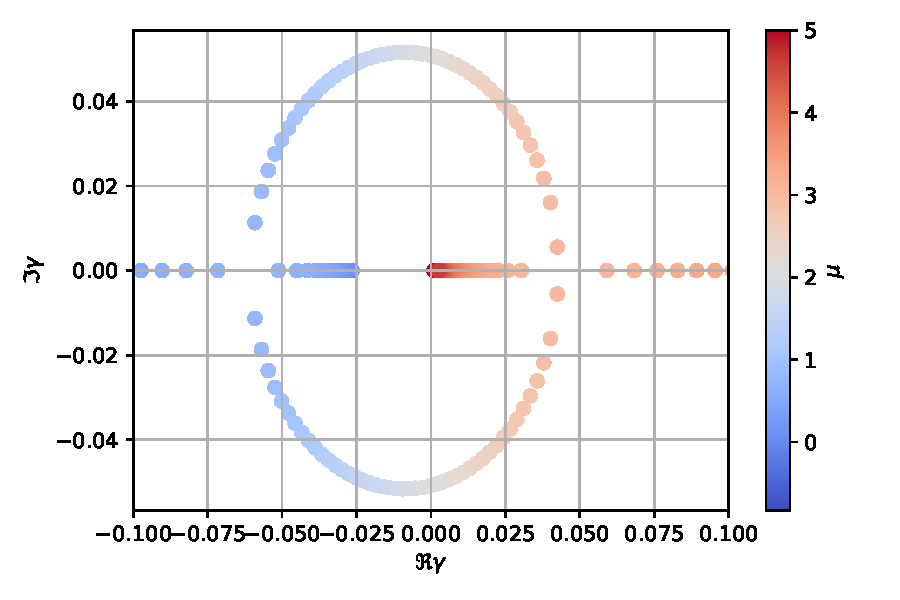
\includegraphics[width=\textwidth,keepaspectratio]{complex_plane_two_box_eig}
  \caption[Eigenvalues of the two box Jacobian]{The eigenvalues of the Jacobian of the two box model \cref{eq:two_box_ocean} plotted in the complex plane as a
    function of $\mu$.  The colour of the eigenvalue is given
    by the value of $\mu$. The colour scheme has been chosen so that the colours transition from blue to red at the bifurcation point $\mu_-$ given by
  \cref{eq:mu_two_box}. This shows the eigenvalues crossing the imaginary axis at the predicted point, which is where the Hopf Bifurcation happens.}
  \label{fig:eigen_values_of_the_jacobian}
\end{figure}
\begin{figure}
  \centering
  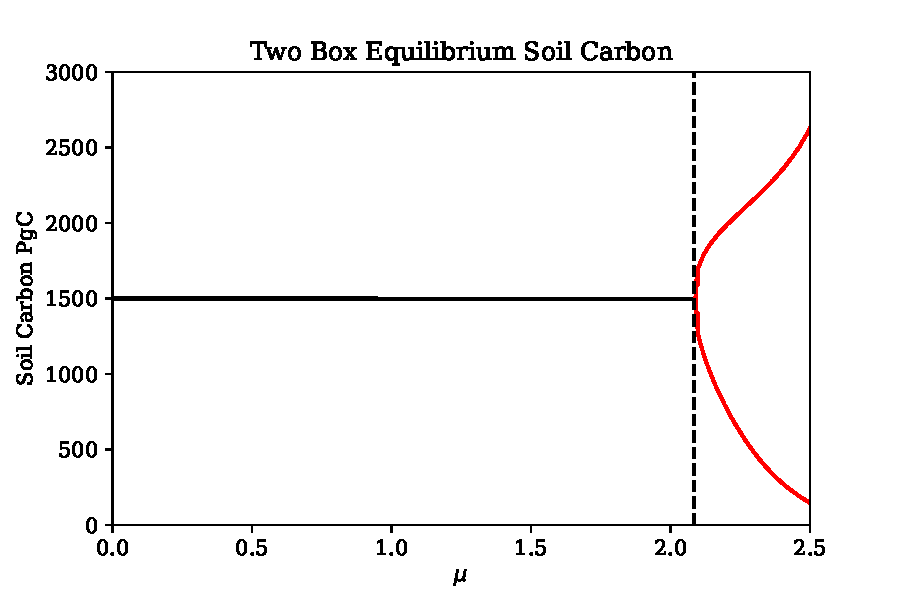
\includegraphics[keepaspectratio,width=\textwidth]{two_box_model_soil_carbon_equilibrium}
  \caption[Two box soil carbon equilibrium]{Equilibrium levels of soil carbon as a function of $\mu$ for the two box ocean model, \cref{eq:two_box_ocean},
    calculated numerically. The ocean parameters are $\tau = \SI{0.45}{\year},\epsilon=0.004$ and $f = 0.5$.
    The dashed line is the analytically calculated bifurcation point, $\mu_-$ given by \cref{eq:mu_two_box}.
  Solid black lines represent a steady state condition, whereas red lines show the maximum and minimum of an oscillatory state. The oscillation period increases almost
    linearly with $\mu$ from around \SI{23}{\year} to \SI{64}{\year}.}
  \label{fig:two_box_bf_diagram}
\end{figure}
Furthermore, the equilibrium soil carbon state is plotted in \cref{fig:two_box_bf_diagram}. It can be seen that the bifurcation corresponds to the theoretical prediction.
No bifurcation was found at $\mu_+$. This could be because $\mu_+$ represents a spurious solution. Alternatively there could be other
parameters for which $\mu_+$ represents a real bifurcation. In any case as $\mu_+ > \mu_-$, the bifurcation at $\mu_-$ will have more relevance to the climate system.

It can be seen therefore that the two box model is complex enough to reproduce the behaviour of the IMOGEN model but simple enough to be analytically tractable.

\section{Model Comparison}
In this chapter, the ocean component of the Earth's carbon cycle has been represented in three different ways: by a one-box, a two-box and as a more complex model. Each model suggests the carbon cycle
has bifurcations for large enough values of the climate sensitivity. In this next figure, \cref{fig:imogen_one_box_two_box} the equilibria are plotted for each model.
\begin{figure}
  \centering
  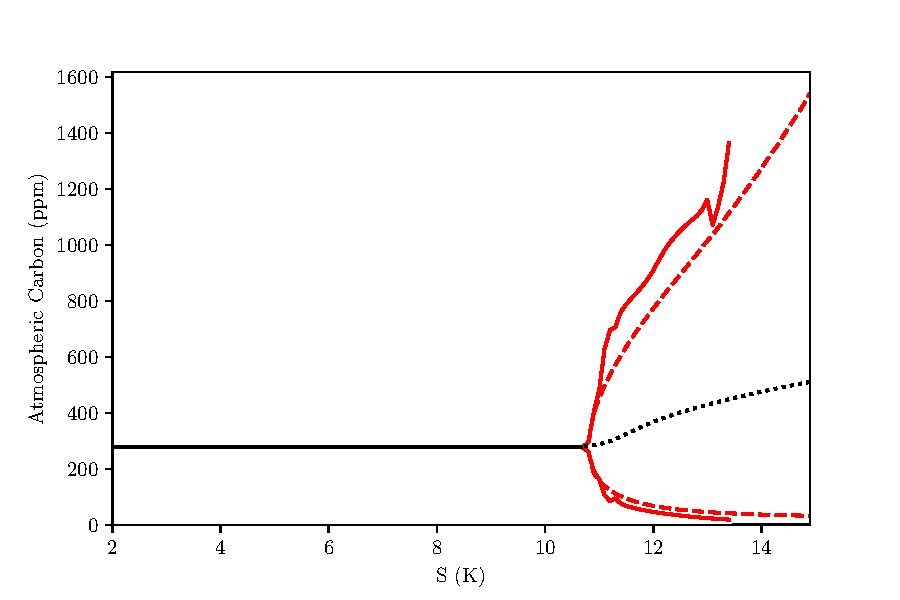
\includegraphics[keepaspectratio,width=\textwidth]{imogen_one_box_two_box}
  \caption[Comparison of bifurcation diagrams for IMOGEN, one and two box ocean carbon cycle models]{A comparison of the bifurcation diagrams of the IMOGEN,
    one box and two box models. Ocean parameters have been chosen so that the bifurcation happens at the same value of $S$.
    $Q_{10}$ has been set to $2$. Black lines represent a steady state condition, whereas red lines show that maximum and minimum of an oscillatory state.
    The solid lines are the values for IMOGEN, the dotted lines are for the one box model and the dashed lines are for the two box model. IMOGEN and the two box model
    undergo a Hopf bifurcation at $S \approx \SI{10.5}{\kelvin}$, whereas the one box model undergoes a transcritical bifurcation here. The oscillation period for the two box model
    increases linearly with $S$ from \SI{34}{\year} to \SI{77}{\year}. The oscillation period for the IMOGEN model shows little variation with $S$, having an oscialltion period of \SI{1250}{\year}.}
\label{fig:imogen_one_box_two_box}
\end{figure}
The ocean parameters have been chosen so that the bifurcation occurs at the same point. For the one box model, this involved setting $\tau = \SI{2.34}{\year}$. For the two box model there
was more freedom in the parameter choice. The choice $\tau_1 = \SI{0.1}{\year}$, $f = 0.92$ and $\epsilon = 1.6\times 10^{-5}$ was made.

Unlike the other two models, the one box model does not give any oscillatory behaviour. The two box model gives  oscillations for all values of $S$ above a threshold, whereas IMOGEN shuts the
oscillations down at large enough $S$, and no carbon is found in the atmosphere. However the two box model and IMOGEN give qualitative agreement on the amplitude of the limit cycles beyond the bifurcation
point.

\subsection{Ocean Parameter Estimation}
\label{sec:ocean_uptake}
\Cref{eq:ocean_response} can be fitted to observed changes in ocean carbon to estimate the
parameters $f_i$ and $\tau_i$ in the $N$-box models. This is done for the one box model, in which only $\tau_1$ needs to be estimated and
for the two box model where $\tau_1$,$\tau_2$ and $f_1$ must be estimated. The quantity $f_2$ is determined by the requirement that $f_1 + f_2 = 1$.
\begin{table}
  \centering
  \begin{tabular}{@{}lll@{}}
    \toprule
    \multicolumn{1}{c}{Parameter} & \multicolumn{2}{c}{Estimated Quantity} \\
    \cmidrule{2-3}
                                  & One Box         & Two Box              \\
    \midrule
    $\tau_1$                      & \SI{3.7}{\year} & \SI{0.5}{\year}      \\
    $\tau_2$                      &                 & \SI{124}{\year}      \\
    $f_1$                         & $1$             & $0.9$                \\
    $f_2$                         & $0$             & $0.1$                \\
    \bottomrule
  \end{tabular}
  \caption{Parameter Estimates for one and two box ocean models.}
  \label{tab:one_and_two_box_parameters}
\end{table}

Using \cref{eq:ocean_response}, the ocean carbon uptake for an atmospheric \ce{CO2} time series can be computed for given values of $\tau_i$ and $f_i$.
The Global Carbon Budget \parencite{Friedlingstein2022} provide estimates of the ocean carbon uptake as well as the increase atmospheric carbon
dioxide, which is ultimately caused by anthropogenic activities, from the year 1781 onwards. Assuming $\Delta C_o = \Delta C_a = 0$ before 1781, a least squares fit of the
Global Carbon Budget data can be performed to \cref{eq:ocean_response} to estimate the parameters $\tau_1$ for the one box model, and $\tau_1,\tau_2$ and $f_1$ for the two box model.
These parameter estimates are shown in \cref{tab:one_and_two_box_parameters}.

\begin{figure}
  \centering
  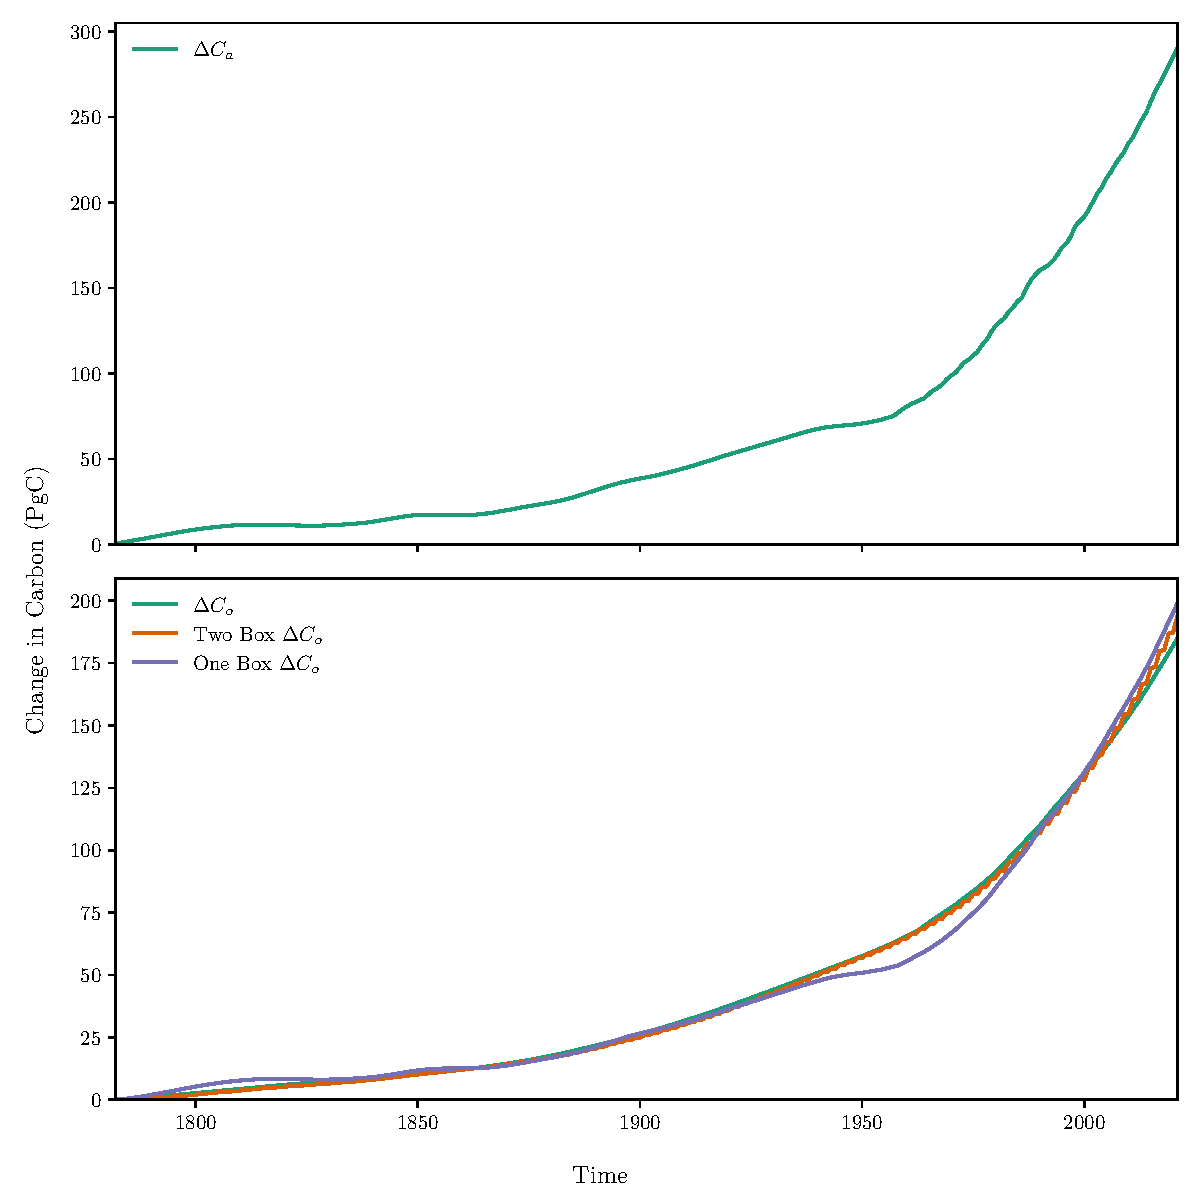
\includegraphics[keepaspectratio,width=\textwidth]{gcb_ocean_atmosphere_boxes}
  \caption[One and two box fits to observations]{The fit of \cref{eq:ocean_response} to the ocean carbon uptake estimated by the Global Carbon Budget using one and
    two box models. The fitted parameters are given in
    \cref{tab:one_and_two_box_parameters}. The driving atmospheric \ce{CO2} is plotted in the top panel, and the ocean uptake in the lower panel. Both one and two boxes give decent fits
    to the data but the two box model gives a better fit.}
  \label{fig:fits_from_one_and_two}
\end{figure}

These fits are plotted in \cref{fig:fits_from_one_and_two}. It can be seen that both one and two box models do a reasonable job in capturing the
historical record of ocean carbon uptake. However the two box model does better, although this to to be expected given the two extra parameters.

These parameters can also be compared to the ones used to make the bifurcation point in IMOGEN line up with the bifurcation points in the one and two box models. In the one box model case,
the single parameter $\tau_1$ is close to that used to match the IMOGEN case. In the two box case, parameters $\tau_1$ and $f_1$ are similar, however the second timescale obtained from observations
is much shorter.

\section{Conclusion}
In this chapter I have taken a simple but physically motivated model of the carbon cycle and shown that only certain parameter values are compatible with the qualitative behaviour
of the terrestrial carbon cycle during the Holocene. In particular these parameters relate to key sensitivities in the Earth system: the climate sensitivity, the sensitivity of
terrestrial carbon to temperature and the sensitivities of net primary production to \ce{CO2}. In this model I find that the negative feedbacks on the system (namely changes in net primary
production due to increased \ce{CO2}) must be sufficiently strong enough to offset the positive feedbacks (the Jenkinson effect).

For realistic parameters of $Q_{10} = 2$ and $C_{1/2} = \SI{280}{\ppm}$, the critical value of $S$ which leads to an instability is \SI{10.7}{\kelvin}.
This is similar to, but larger than, the~\cite{Cox2006} critical value of \SI{9}{\kelvin}, a difference which can be attributed to the simplified representation of the ocean in that paper.

Although this model was relatively simple, the ocean component is still too complex to handle analytically. I simplified the ocean model down to a box model of the oceans,
which meant I could derive exact results about the bifurcation. I found that a single box could recreate the oscillatory behaviour seen for large enough climate sensitivities,
however it did not do this at the correct bifurcation point. On the other hand, a two box model could reproduce the oscillations at the correct bifurcation point.

I could then fit the box models to the observed carbon uptake by the oceans to estimate what parameters best fit the observations. These parameters are similar to those found in the more
complex model, although they disagree on the position of the bifurcation.